\chapter{Produtos, Atividades e Cronograma}

\section{Resumo da Proposta}
	O processo de medição será realizado sobre o objeto da disciplina de Introdução a Jogos Eletrônicos. Neste objeto serão realizados processos de medição no contexto do produto e da equipe de desenvolvimento. O processo de medição será iniciado juntamente com o desenvolvimento do projeto, podendo dessa forma auxiliar ativamente a equipe a melhorar seu processos administrativos e de desenvolvimento.
	
	A medição será iniciada com o levantamento dos objetivos de negócio, que representam as metas buscadas pela equipe no desenvolvimento do jogo. Com os objetivos definidos serão levantadas questões que auxiliarão na descoberta de elementos, métricas, que podem ajudar a concretizar os objetivos estabelecidos.

	A avaliação da disciplina de Introdução aos Jogos Eletrônicos será avaliada em marcos, indicando também quando serão coletados os dados relacionados a medição do processo de desenvolvimento, sendo eles:

	\begin{itemize}
		\item Marco 1: 19/04 (Esse marco não será medido, pois será apenas apresentação da ideia do jogo)
		\item Marco 2: 05/05/2017
		\item Marco 3: 31/05/2017
		\item Marco 4: 21/06/2017
		\item Marco 5: 07/07/2017 - Apresentação do jogo completo
	\end{itemize}
	
\section{Estrutura Analítica do Projeto}
	\begin{figure}[!htpb]
		\centering
		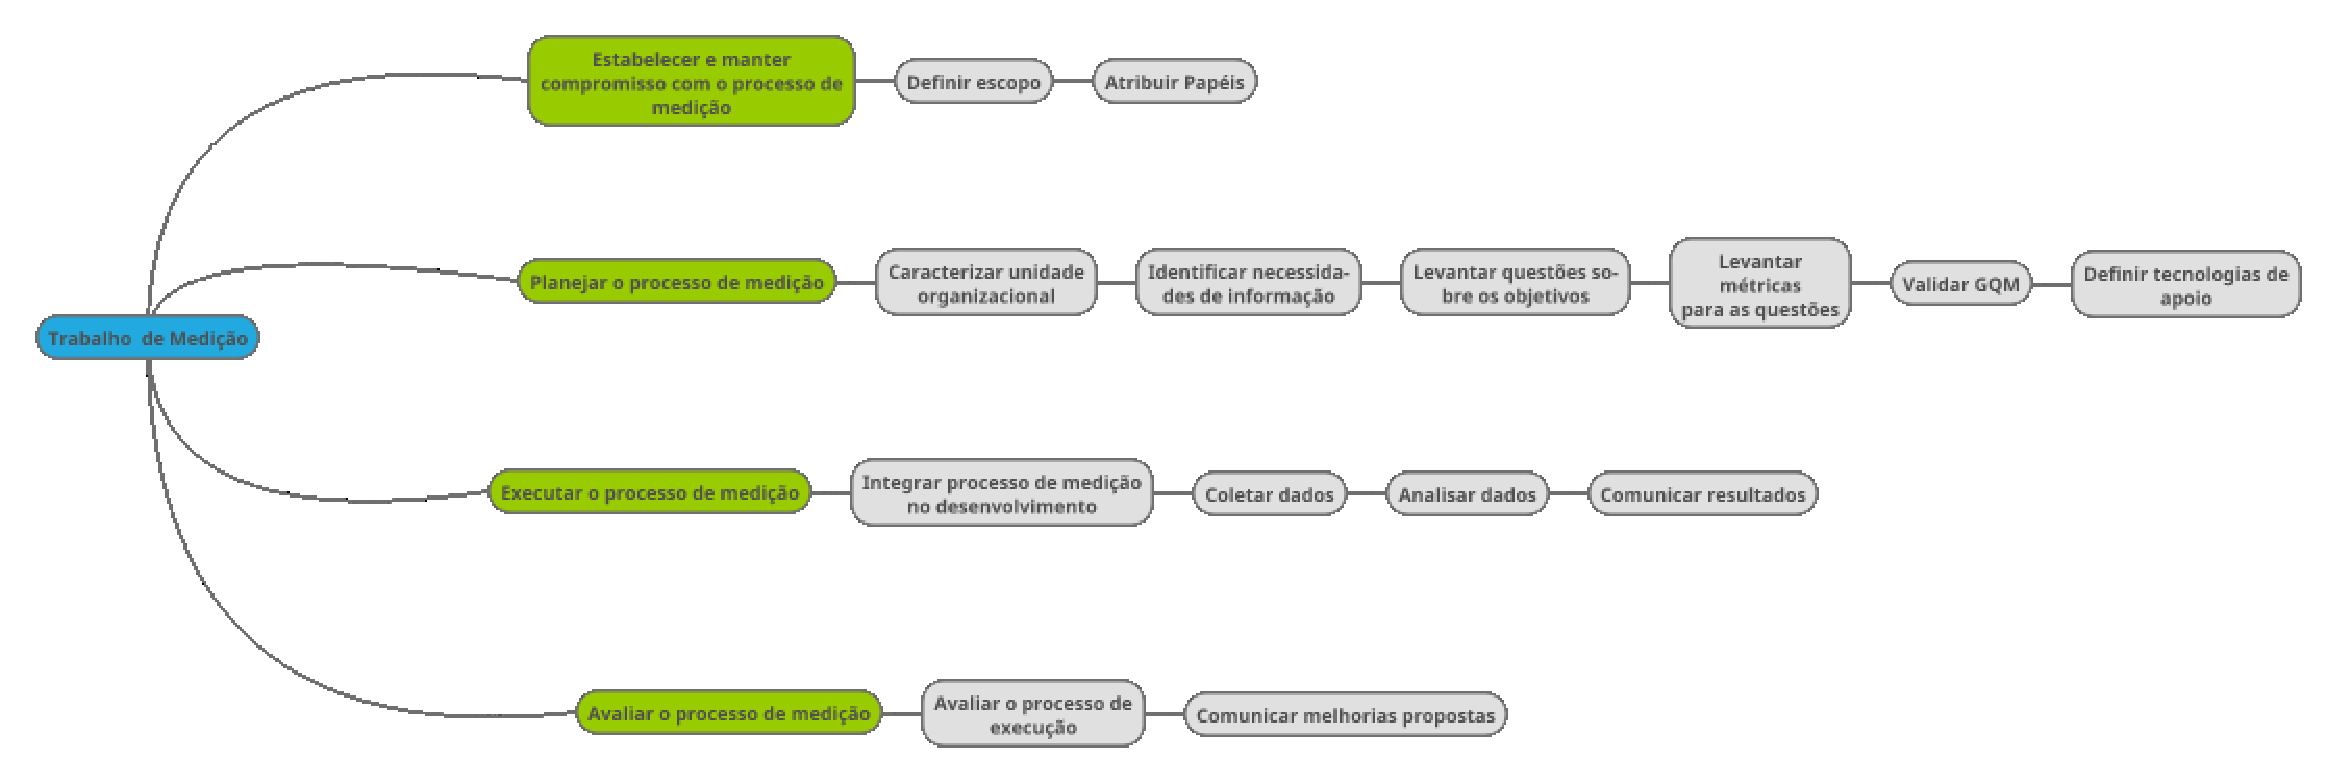
\includegraphics [scale=0.35]{figuras/processo/eap}
		\caption{Estrutura Analítica do Projeto}
	\end{figure}
	
\section{Lista de Software}
	As ferramentas necessárias para o desenvolvimento do produto de software da disciplina de Introdução a Jogos Digitais serão: 
	\begin{itemize}
		\item Ferramenta de Gerenciamento de Versão Git

	\end{itemize}
	
	As ferramentas utilizadas pela equipe de medição para auxiliar na coleta de métricas e para produção da documentação serão:
	
	\begin{itemize}
		\item Draw.io para produção dos modelos de processo e diagramas
		\item Simian e cLint para coleta de métricas relacionadas ao desenvolvimento do software
		\item Wakatime para coleta de métricas relacionadas a produção de artefatos
	\end{itemize}
	
\section{Cronograma}
	O cronograma foi utilizado para organizar os processos da primeira e da segunda entrega relacionados ao projeto de medição em formato sequencial, bem como definir quais os integrantes participarão de cada atividade e o tempo de duração das mesmas.
	\begin{figure}[!htpb]
		\centering
		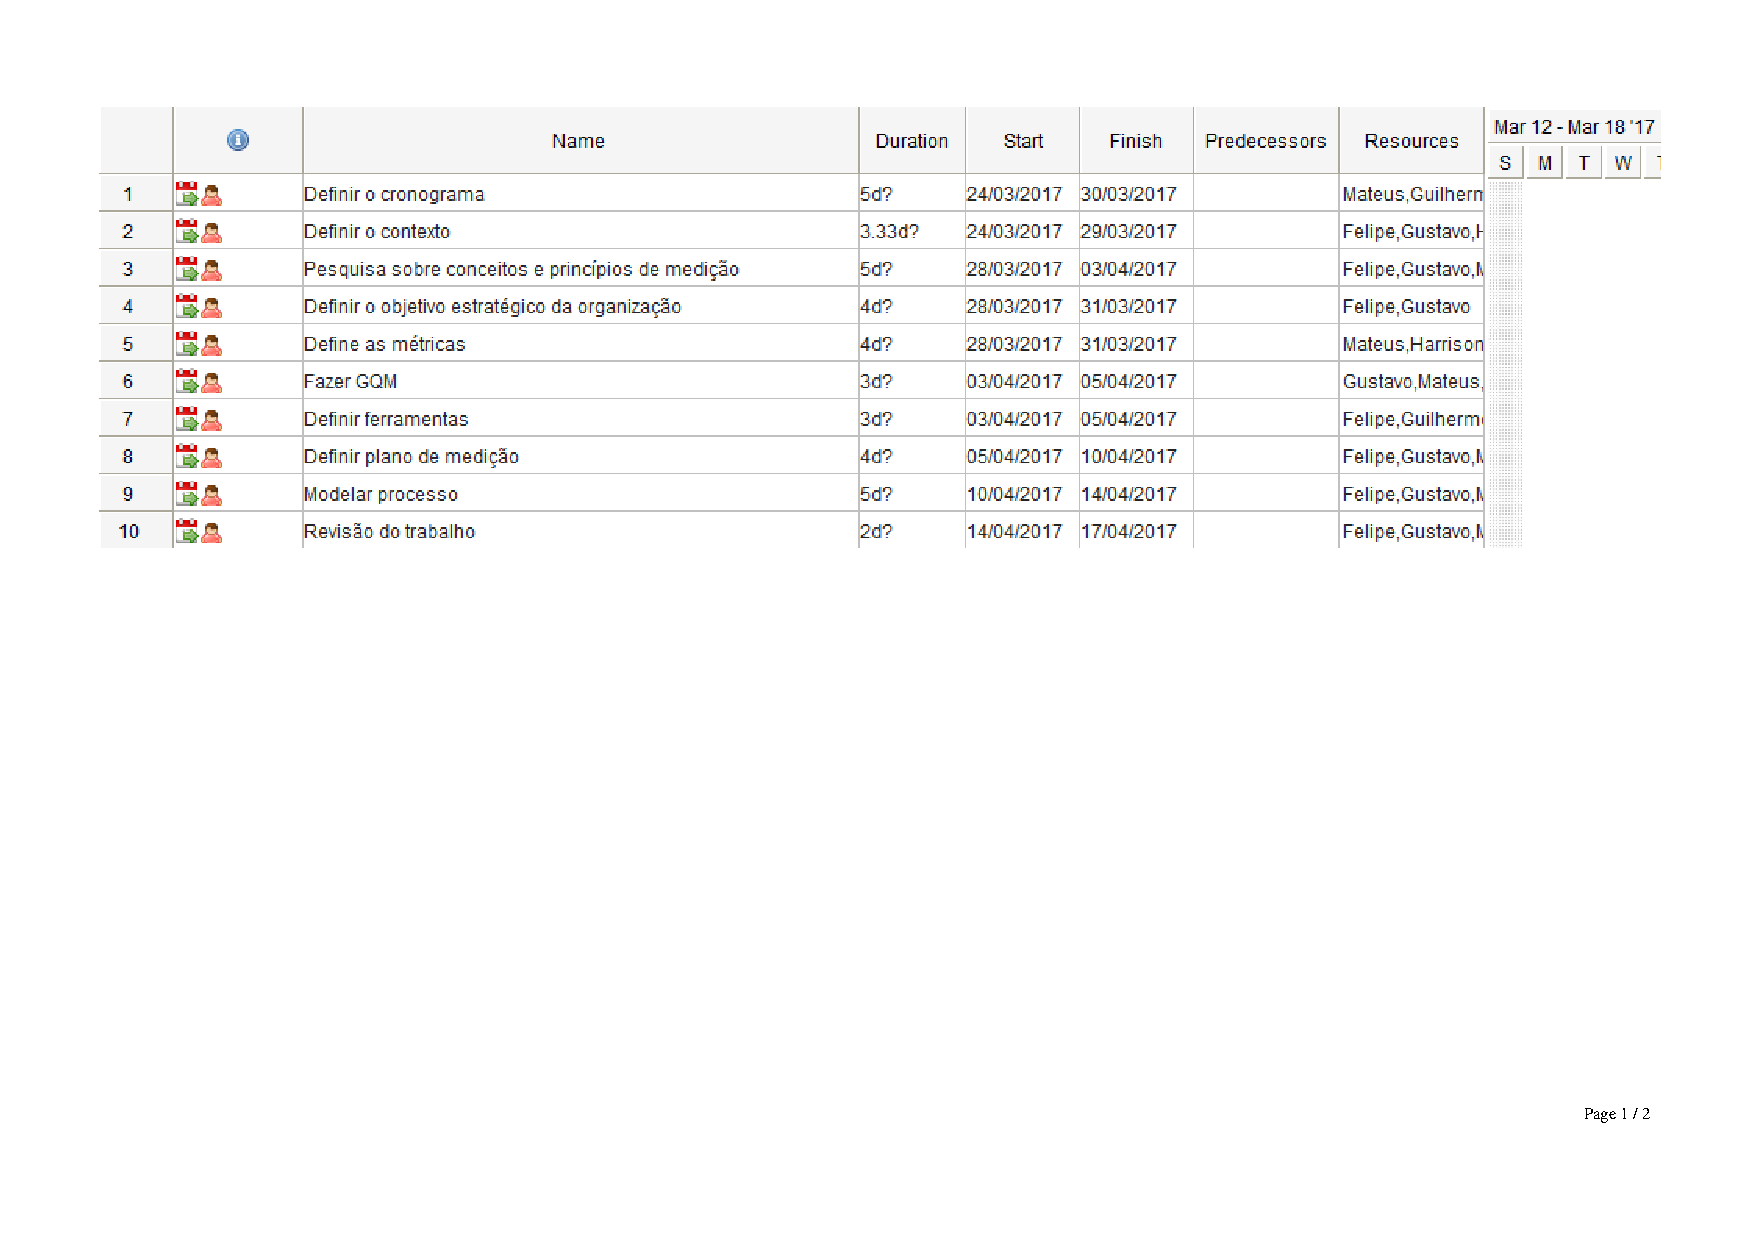
\includegraphics [scale=0.35]{figuras/processo/cronograma}
		\caption{Cronograma utilizado pela equipe}
	\end{figure}
	\newpage
\section{Descrição das Atividades}

Nessa seção serão descritas a atividades elustradas no processo no capítulo 4 deste relatório, separando cada atividade de acordo com as fases relatadas na ISO/IEC/IEEE 15939:2008, descrevendo e indicando os responsáveis sobre as mesmas.

\subsection{Fase 1 - Estabelecer e manter compromisso com o processo de medição}
	\begin{tabular}{ |p{4cm}|p{6cm}| p{3cm} |}
	 \hline
	 Atividade 		& 		Descrição & Responsáveis \\
	 \hline
	 	Definir Escopo & x &  y \\
	 \hline
	 	Definir papéis & x &  y \\
	 \hline
	\end{tabular}


\subsection{Fase 2 - Planejar o processo de medição}

	\begin{tabular}{ |p{4cm}|p{6cm}| p{3cm} |}
	 \hline
	 Atividade 		& 		Descrição & Responsáveis \\
	 \hline
	 	Caracterizar unidade organizacional & x &  y \\
	 \hline
	 	Identificar necessidades de informação & x &  y \\
	 \hline
	 	Levantar questões sobre os objetivos & x &  y \\
	 \hline
	 	Levantar questões sobre os objetivos & x &  y \\
	 \hline
	 Levantar métricas para as questões & x &  y \\
	 \hline
	 Validar GQM & x &  y \\
	 \hline
	 Definir tecnologias de apoio & x &  y \\
	 \hline
	\end{tabular}

\subsection{Fase 3 - Executar o processo de medição}

	\begin{tabular}{ |p{4cm}|p{6cm}| p{3cm} |}
	 \hline
	 Atividade 		& 		Descrição & Responsáveis \\
	 \hline
	 	Integrar processo de medição no desenvolvimento & x &  y \\
	 \hline
	 	Coletar Dados & x &  y \\
	 \hline
	 	Analisar os Dados & x &  y \\
	 \hline
	 	Comunicar resultados & x &  y \\
	 \hline
	\end{tabular}

\subsection{Fase 4 - Avaliar o processo de medição}

	\begin{tabular}{ |p{4cm}|p{6cm}| p{3cm} |}

	 \hline
	 Atividade 		& 		Descrição & Responsáveis \\
	 \hline
	 	Avaliar o processo de execução & x &  y \\
	 \hline
	 	Comunicar melhorias propostas & x &  y \\
	 \hline

	\end{tabular}
